% \documentclass{beamer}
%Information to be included in the title page:
%\title{Moufangové rovina a spinové grupy}
%\author{Dominik Stejskal}
% \institute{Overleaf}
%\date{1. 4. 2022}

% test change after setting up offline backup

\documentclass[9pt]{beamer}

\usepackage{times,color}
\usepackage[czech]{babel}
\usepackage[utf8]{inputenc}
\usepackage{amsmath}
\usepackage[cmtip,all]{xy}
\usepackage[T1]{fontenc}
\usepackage[normalem]{ulem}

\usepackage{mathtools}   % přidal jsem já...
\usepackage[bb=stix]{mathalpha}  % KVŮLI LOWERCASE BBM A PDF/A-2u
\usepackage{todonotes}
\setuptodonotes{inline}  % CUSTOMIZACE TODONOTES
\usepackage{bm}
\usepackage{xcolor}         % typesetting in color

%%%%%% my own macros section %%%%%%%%%%%%%%%%%%%%%
\newcommand{\red}[1]{\textcolor{red!}{#1}}

\newcommand{\R}{\mathbb{R}}
\newcommand{\N}{\mathbb{N}}
\newcommand{\Z}{\mathbb{Z}}
\newcommand{\Q}{\mathbb{Q}}
\newcommand{\q}{\mathbb{q}}
\newcommand{\F}{\mathbb{F}}
\newcommand{\G}{\mathbb{G}}
\newcommand{\e}{\hat{e}}

\newcommand{\probability}[2]{
    \Pr
    \left[ 
    \begin{aligned}
    #1 \mspace{1mu}
    \end{aligned}
    \middle\vert
    \begin{aligned}
    \mspace{2mu} #2
    \end{aligned}
    \right]
}

\newcommand{\poly}{\mathsf{poly}}
\newcommand{\Pgen}{\mathsf{PGen}}
\newcommand{\KGen}{\mathsf{KGen}}
\newcommand{\Com}{\mathsf{Com}}
\newcommand{\Open}{\mathsf{Open}}
\newcommand{\V}{\mathsf{Vrf}}  % verification
\newcommand{\Ext}{\mathsf{Ext}}  % extractor
\newcommand{\Rev}{\mathsf{Rev}}  % revealer
\newcommand{\ck}{\mathsf{ck}}  % commitment key
\newcommand{\negligible}{\approx_{\lambda} 0}
\newcommand{\A}{\mathcal A}  % adversary
\newcommand{\B}{\mathcal B}  % adversary
\newcommand{\RND}{\mathsf{RND}_\lambda}  % random tape
\newcommand{\gp}{\mathsf{gp}}  % group parameters
\newcommand{\Oracle}{\mathcal{O}}  % oracle
\newcommand{\EF}{\mathcal{EF}}  % family of functions
\newcommand{\DF}{\mathcal{DF}}  % family of distributions
\newcommand{\il}{\mathsf{il}}  % input length
\newcommand{\ol}{\mathsf{ol}}  % output length
\newcommand{\ql}{\mathsf{ql}}  % query length
\newcommand{\fpr}{\mathsf{fpr}}  % find polynomial representation
\newcommand{\tofr}{\mathsf{tofr}}  % find polynomial representation
\DeclareMathOperator{\vectorization}{vec}
\newcommand{\Vexpl}{V^\mathsf{expl}}  % explicit verification polynomial
\newcommand{\caseA}{\ensuremath{\mathsf{A}}}
\newcommand{\caseQ}{\ensuremath{\mathsf{Q}}}
\newcommand{\caseX}{\ensuremath{\mathsf{X}}}
\newcommand{\caseXone}{\ensuremath{\mathsf{X.1}}}
\newcommand{\caseXtwo}{\ensuremath{\mathsf{X.2}}}

%%%%%%%%%%%%%%%%%%%%%%%%%%%%%%%%%%%%%%%%%%%%%%%%%%%%%%%%%%%%%%%%%%%%%%%%%

\newtheorem{proposition}{Proposition}
%\newtheorem{theorem}{Theorem}
%\newtheorem{lemma}{Lemma}
%\newtheorem*{example}{Example}
\mode<presentation>
{
  \usetheme{Warsaw}
  \title{On the power of algebraic group models}
  \author{Dominik Stejskal}
  \date{Supervisor: Mgr. Pavel Hubáček, Ph.D.\\ \, \\2 June 2025}
}

%%%%%%%%%%%%%%%%%%%%%%%%%%%%%%%%%%%%%%%%%%%%%%%%%%%%%%%%%%%%%%%%%%%%%%

\begin{document}

\frame{\titlepage}




\begin{frame}
\frametitle{Overview}
\begin{itemize}
    \item Polynomial Commitment Schemes (PCSs)
    \item Algebraic Group Model (AGM)
    \item Algebraic Group Model with Oblivious Sampling (AGMOS)
\end{itemize}
\end{frame}


\begin{frame}
\frametitle{Preliminaries}
\begin{itemize}
    \item Security parameter $ \lambda $
    \item Group parameters 
    \[
    \Pgen(1^\lambda) \to \gp = (p, \G_1, \G_2, \G_T, [1]_1, [1]_2, [1]_T, \hat e)
    \]
    \item $ p $ a prime %, $ \F = \Z_p $
    \item $ (\G_1, +) $, $ (\G_2, +) $, $ (\G_T, +) $ cyclic groups of order $ p $
    \item $ \bullet \colon \G_1 \times \G_2 \to \G_T $, $ (g, h) \mapsto g \bullet h $ a \textit{pairing}, i.e., a non-degenerate, efficiently computable bilinear map
    \item For $ \kappa \in \{ 1, 2, T \} $, $ a \in \F $ and $ \mathbb b \in \F^n $, let $ [a]_\kappa = a[1]_\kappa \in \G_\kappa $, 
    \[ 
    [\mathbb b]_\kappa = [b_1, \dots, b_n]_\kappa = ([b_1]_\kappa, \dots, [b_n]_\kappa) \in \G_\kappa^n
    \]
    \todo{maybe only mention negligible fn when it is used (once)?}
    \item A \textit{negligible function} approaches $ 0 $ faster than any inverse polynomial: $ \phi(\lambda) \negligible $
\end{itemize}
\end{frame}


\begin{frame}
\frametitle{Polynomial Commitment Schemes (PCSs)}
    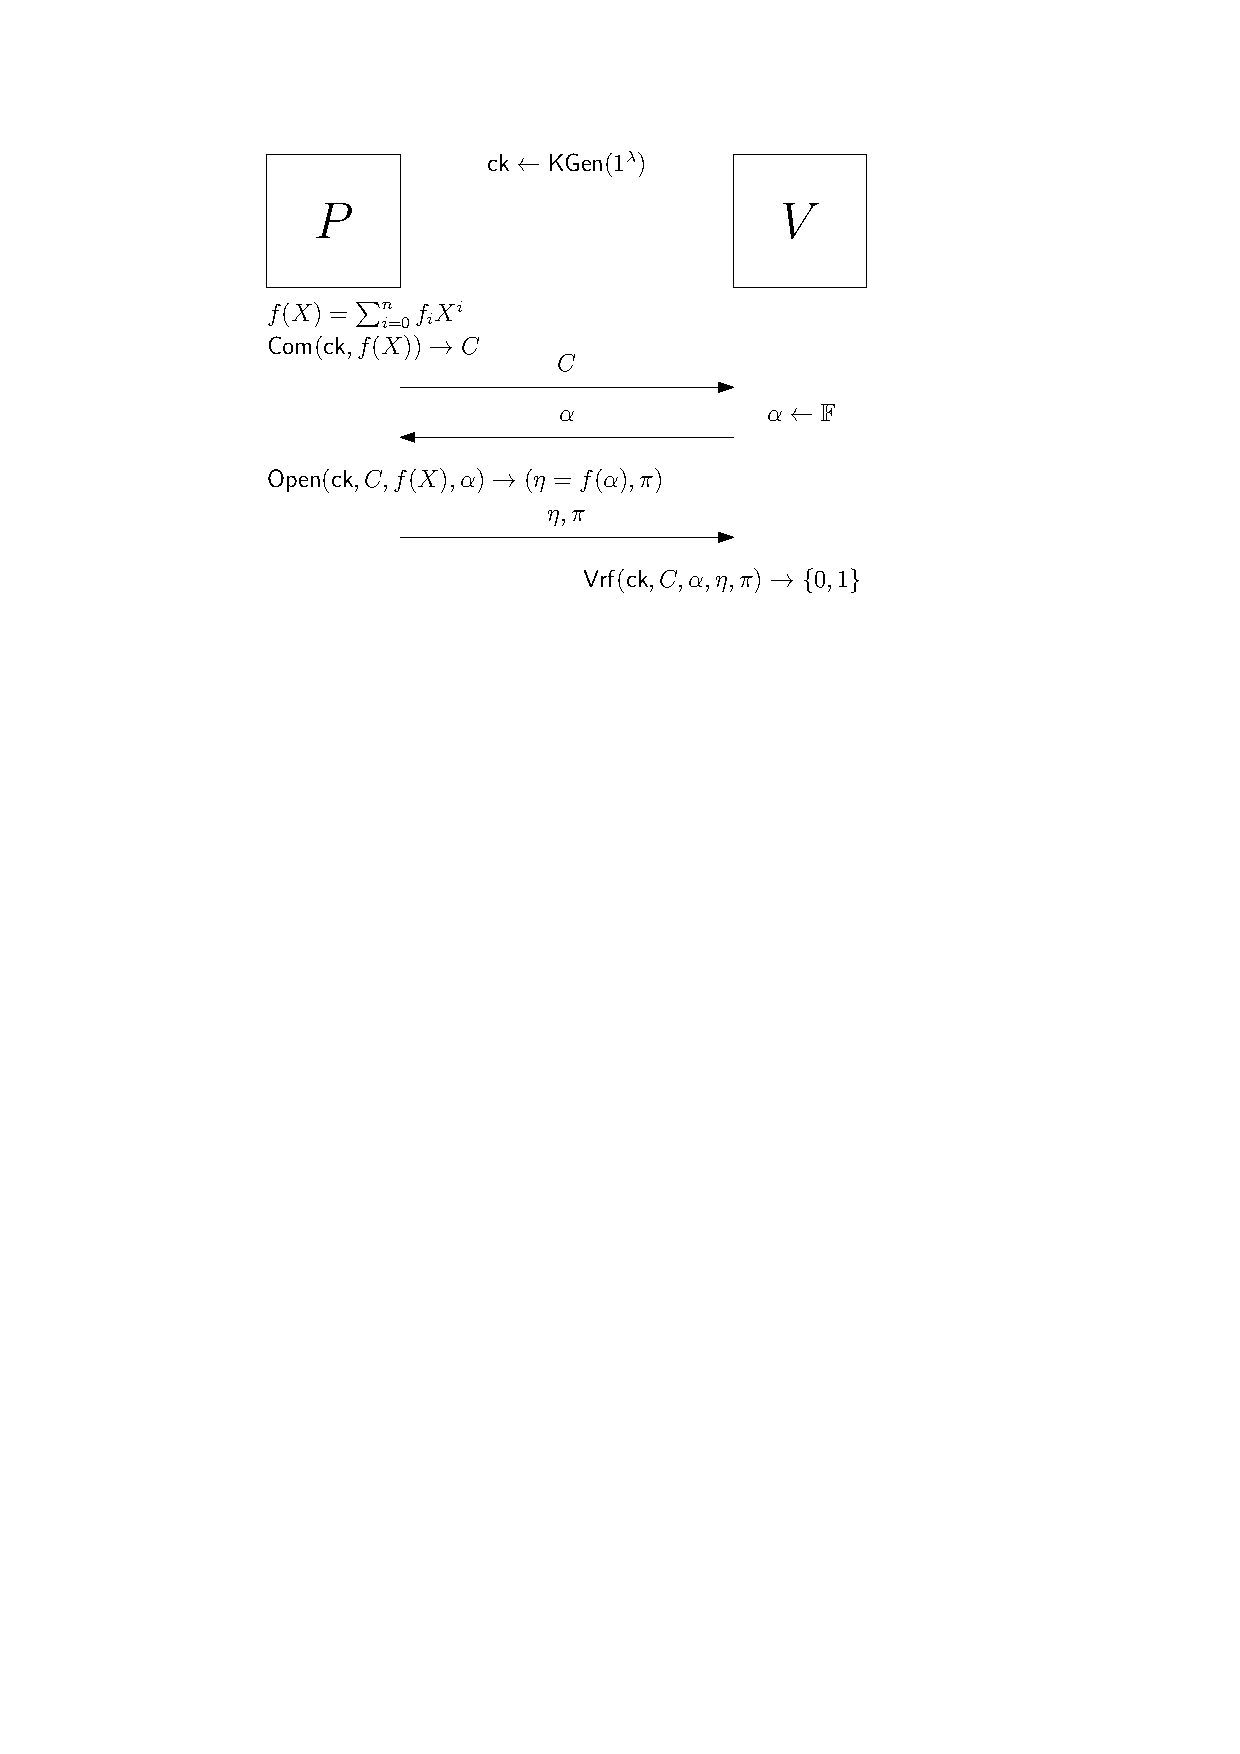
\includegraphics[width=10cm]{pcs-definition.pdf}
\end{frame}


\begin{frame}
\frametitle{Kate-Zaverucha-Goldberg (KZG)}
    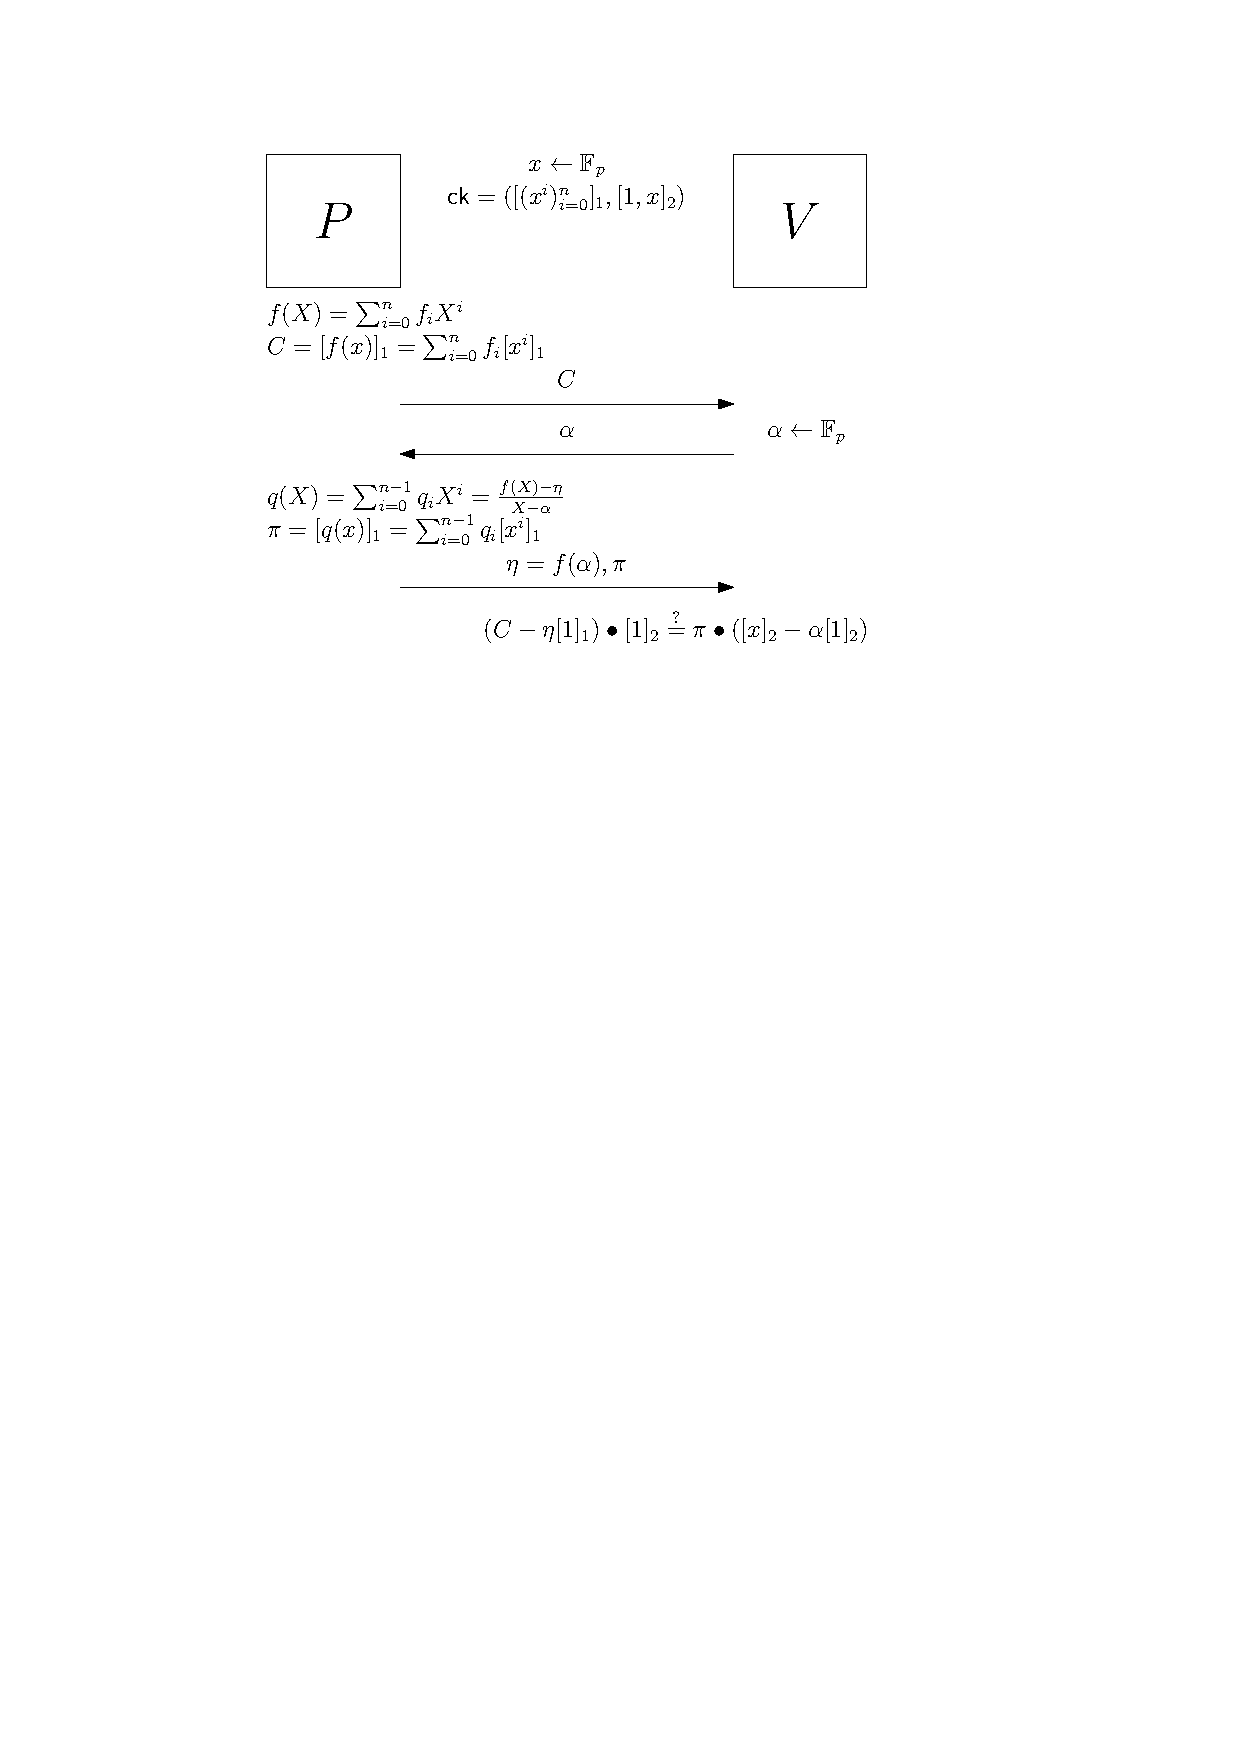
\includegraphics[width=10cm]{kzg.pdf}
\end{frame}


\begin{frame}
\frametitle{Security properties of PCSs}
\todo{too long?}
\begin{definition}
    A PCS is \emph{evaluation binding} if for any $ n \in \poly(\lambda) $ and PPT adversary $ \A $, 
    $$
    \probability{
    & \V(\ck, C, \alpha, \eta, \pi) = 1 \; \land \\ 
    & \V(\ck, C, \alpha, \eta', \pi') = 1 \; \land \\ 
    & \; \eta \neq \eta'
    }{
    & \gp \leftarrow \Pgen(1^\lambda); \ck \leftarrow \KGen(\gp, n); \\
    & (C, \alpha, \eta, \pi, \eta', \pi') \leftarrow \A(\ck)
    }
    \negligible.
    $$
\end{definition}
Intuition: it is hard to prove the nonsensical claim that $ \eta = f(\alpha) = \eta' \neq \eta $.
\begin{definition}[informal]
    A PCS is \textit{extractable} if, for every PPT adversary $ \A $, there exists a PPT \textit{extractor} $ \Ext_{\A} $ satisfying the following. If $ \A $'s output passes the PCS verification, then $ \Ext_\A $, given ``access'' to $ \A $, ``extracts'' the committed polynomial $ f(X) $.
\end{definition}
Intuition: a successful prover must be ``thinking of $ f(X) $ in its head''.
\end{frame}


\begin{frame}
\frametitle{Algebraic Group Model (AGM)}
\todo{do I have to mention GGM?}
\begin{itemize}
    \item Fuchsbauer, Kiltz, and Loss, 2017
    \item Every PPT adversary is \textit{algebraic}:
    $$
    \A(\gp, [\mathbb x_1]_1, [\mathbb x_2]_2) \to (([\mathbb y_1]_1, \bm \gamma_1), ([\mathbb y_2]_2, \bm \gamma_2)),
    $$
    where $ \bm{\gamma}_1 $, $ \bm{\gamma}_2 $ are matrices over $ \F $, and it holds that 
    \begin{equation*}
    \mathbb y_1 = \bm{\gamma}_1 \mathbb x_1, \quad 
    \mathbb y_2 = \bm{\gamma}_2 \mathbb x_2. 
    \end{equation*}
\end{itemize}
\begin{proposition}
    In the AGM, the discrete logarithm assumption and the computational Diffie-Hellman assumption are equivalent.
\end{proposition}
\end{frame}


\begin{frame}
\frametitle{Extractability in the AGM}
In the AGM,
\[
\A(\ck) \to ((C, \bm \gamma_C), \alpha, \eta, (\pi, \bm \gamma_\pi)),
\]
where 
\[
C = \sum_{i=0}^n {\gamma_C}_i [x^i]_1 = 
\left[ \sum_{i=0}^n {\gamma_C}_i x^i \right]_1 = 
\Com(\ck, f)
\]
for $ f(X) = \sum_{i=0}^n {\gamma_C}_i X^i $.

Building on the ideas of P.\ Chmel, C.\ Hoffmann and P.\ Hubáček:
\begin{theorem}[informal]
In the AGM, if a ``\textbf{KZG-like}'' PCS is evaluation binding, then it is extractable.
\end{theorem}
Conclusion: the AGM is likely not suitable for proving extractability. 
\end{frame}


\begin{frame}
\frametitle{Algebraic Group Model with Oblivious Sampling (AGMOS)}
\todo{todo: zopakovat slide bez červené barvy?}
\begin{itemize}
    \item Lipmaa, Parisella, and Siim, 2023 [LPS23]
    \item Oblivious sampling oracle $ \Oracle(\kappa, E, D) \to [q]_\kappa \in \G_\kappa $, where $ \kappa \in \{ 1, 2 \} $.
    \item \(
    \A^{\red{\Oracle}}(\gp, [\mathbb x_1]_1, [\mathbb x_2]_2) \to
    ([\mathbb y_\kappa]_\kappa, \bm \gamma_\kappa, \red{\bm \delta_\kappa}, \red{[\mathbb q_\kappa]_\kappa})_{\kappa=1}^2
    \), where $ \bm{\gamma}_\kappa $, $ \red{\bm{\delta}_\kappa} $ are matrices over $ \F $, and it holds that 
    \begin{equation*}
    \mathbb y_\kappa = \bm{\gamma}_\kappa \mathbb x_\kappa \red{+ \bm \delta_\kappa \mathbb q_\kappa}, \quad 
    \kappa \in \{ 1, 2 \}.
    \end{equation*}
\end{itemize}   
\end{frame}


\begin{frame}
\frametitle{TOFR, FPR assumptions}
\begin{definition}[informal]
    The \emph{Tensor Oracle Find Representation (TOFR)} assumption holds if, for any PPT adversary $ \A $, which receives $ [\mathbb q_1]_1 $, $ [\mathbb q_2]_2 $ from the AGMOS oracle $ \Oracle $, it is ``difficult'' to find $ \bm v \neq \bm 0 $ such that
    \[
    \bm v^T 
    \begin{pmatrix}
         1 \\
         \mathbb q_1 \\
         \mathbb q_2 \\
         \mathbb q_1 \otimes \mathbb q_2
    \end{pmatrix}
    = 0.
    \]
\end{definition}
Find Polynomial Representation (FPR) oracle: $ \bm x \gets \F^m $, 
\[ 
\Oracle^\fpr(\bm x, \kappa, f(\bm X)) \to [f(\bm x)]_\kappa.
\]
\begin{definition}[informal]
    The \textit{FPR assumption} holds if, for any PPT adversary $ \A $ with access to the FPR oracle $ \Oracle^\fpr $, it is ``difficult'' to find $ 0 \neq g(\bm X) $ below a certain degree such that $ g(\bm x) = 0 $.
\end{definition}
\end{frame}


\begin{frame}
\frametitle{AGMOS security game structure}
\begin{itemize}
    \item Trapdoors: $ \bm x \gets \F^m $; formal variables 
    \item Adversary:
    \[
    \A^\Oracle(\gp, [\mathbb x_1(\bm x)]_1, [\mathbb x_2(\bm x)]_2) \to
    (([\mathbb y_\kappa]_\kappa, \bm \gamma_\kappa, \bm \delta_\kappa, [\mathbb q_\kappa]_\kappa)_{\kappa=1}^2, \bm \alpha),
    \]
    where $ \mathbb x_\kappa(\bm X) \in \F[\bm X]^{\il_\kappa} $, $ \bm \alpha \in \F^m $, 
    \[
    \mathbb y_\kappa = \bm{\gamma}_\kappa \mathbb x_\kappa(\bm x) + \bm \delta_\kappa \mathbb q_\kappa, \quad 
    \kappa \in \{ 1, 2 \}.
    \]
    \item Verification (using pairing):
    \[
        \begin{pmatrix}
           \mathbb x_1(\bm x) \\
           \mathbb y_1
        \end{pmatrix}^T
        \bm M
        \begin{pmatrix}
           \mathbb x_2(\bm x) \\
           \mathbb y_2
        \end{pmatrix} \overset{?}{=} 0.
    \]
    Equivalently, $ V(\bm x, \mathbb q) = 0 $ for a certain polynomial
    \[
    V(\bm X, \mathbb Q) = V^h(\bm X) + V^t(\bm X, \mathbb Q).
    \]
\end{itemize}
\end{frame}


\begin{frame}
\frametitle{Main theorem}
Proving that an assumption holds/an algorithm is secure/\dots in the AGMOS. [LPS23] Proof technique:
\begin{itemize}
    \item Case \caseA: $ V(\bm X, \mathbb Q) = 0 $. Impossible, or, for example, the extractor wins.
    \item Case \caseXone: $ V(\bm X, \mathbb Q) \neq 0 $, but $ V^t(\bm X, \mathbb Q) = 0 $. Reduces to FPR.
    \item Case \caseXtwo: $ V^t(\bm X, \mathbb Q) \neq 0 $, but $ V^t(\bm x, \mathbb Q) = 0 $. Reduces (differently) to FPR.
    \item Case \caseQ: $ V^t(\bm x, \mathbb Q) \neq 0 $. Reduces to TOFR.
\end{itemize}
AGM: only cases \caseA \ and \caseXone, since $ V^t(\bm X, \mathbb Q) = 0 $.
\begin{theorem}[informal]
    In the aforementioned AGMOS security game, if $ \A $ passes the verification and the TOFR and FPR assumptions hold, then $ V^t(\bm X, \mathbb Q) = 0 $ with overwhelming probability.
\end{theorem}
\end{frame}


\begin{frame}
\frametitle{AGM to AGMOS ``lifting''}
If $ \A $ outputs $ \bm \delta = (\bm \delta_1, \bm \delta_2) = \bm 0 $, then it is ``basically'' an AGM adversary:
\[
\mathbb y_\kappa = 
\bm{\gamma}_\kappa \mathbb x_\kappa(\bm x) + \bm \delta_\kappa \mathbb q_\kappa = 
\bm{\gamma}_\kappa \mathbb x_\kappa(\bm x), \quad 
\kappa \in \{ 1, 2 \}
\]
Thanks to the main theorem, it remains to show that
\[
V^t(\bm X, \mathbb Q) = 0 \quad \text{implies} \quad
\bm \delta = \bm 0.
\]
LHS is equivalent to a system of polynomial equations which are at most quadratic in $ \bm \delta $. 
\end{frame}


\begin{frame}
\frametitle{Conclusion}
\begin{itemize}
    \item In the AGM, for ``KZG-like'' PCSs, evaluation binding implies extractability. The AGM may not be suitable for proving extractability.
    \item Given an AGM proof of security, extending it to the AGMOS is partially automatized by our main theorem.
\end{itemize}
Thank you for your attention.
\end{frame}


\begin{frame}
\frametitle{???????????????????????????????????????????}
    \todo{Reactions to opponent's review go here.}
\end{frame}


\end{document}